\documentclass[12pt]{report}
\pagenumbering{roman}

%formatting of Source code
\usepackage{listings}
\usepackage{tabularx}
\usepackage{graphicx}
\usepackage{wrapfig} 
\usepackage{subcaption}
\usepackage[utf8]{inputenc}
\usepackage[german]{babel}
% for units
\usepackage{siunitx}
% floats pictures to the correct position when using [H]
\usepackage{float}
\usepackage[hyphens]{url}
\usepackage{hyperref}
\hypersetup{
  colorlinks=true,
  linkcolor=blue,
  filecolor=magenta,      
  urlcolor=cyan,
}

\lstset{frame=tb,
  language=C++,
  aboveskip=3mm,
  belowskip=3mm,
  showstringspaces=false,
  columns=flexible,
  basicstyle={\small\ttfamily},
  numbers=none,
  numberstyle=\tiny\color{gray},
  keywordstyle=\color{blue},
  commentstyle=\color{dkgreen},
  stringstyle=\color{mauve},
  breaklines=true,
  breakatwhitespace=true,
  tabsize=4
}

\urlstyle{same}
\setcounter{chapter}{1}


\begin{document}
% CONSTANTS BEGIN
\newcommand{\paragraphwithnewline}[1]{\paragraph{#1}\mbox{}\\} % used to create a newline after the paragraph tag.
\newcommand{\githubrepo}{\href{https://github.com/Pierrefha/ees-buggy-project}{GitHub-Repository}}

\newcommand{\gquotes}[1]{"`#1"'}
\newcommand{\itoc}{$I^2C$}
\newcommand{\wiringPi}{wiringPi}

% \newcommand{\github_repo}{\href{https://github.com/Pierrefha/ees-buggy-project}{GitHub-Repository}}
% CONSTANTS END
\begin{titlepage}
    \begin{center}
        \Huge
        \textbf{Lernportfolio}

        \normalsize
        \textbf{Pierre Dahmani pd1528s 3215892\\
        Jens Peter Dennigmann jd8389s 3190025 \\
        Leonhard Kipp lk2149s 3188047\\}
            
        \vspace{0.8cm}
            
        \begin{figure}[H]
          \centering
          \captionsetup[subfigure]{labelformat=empty}
          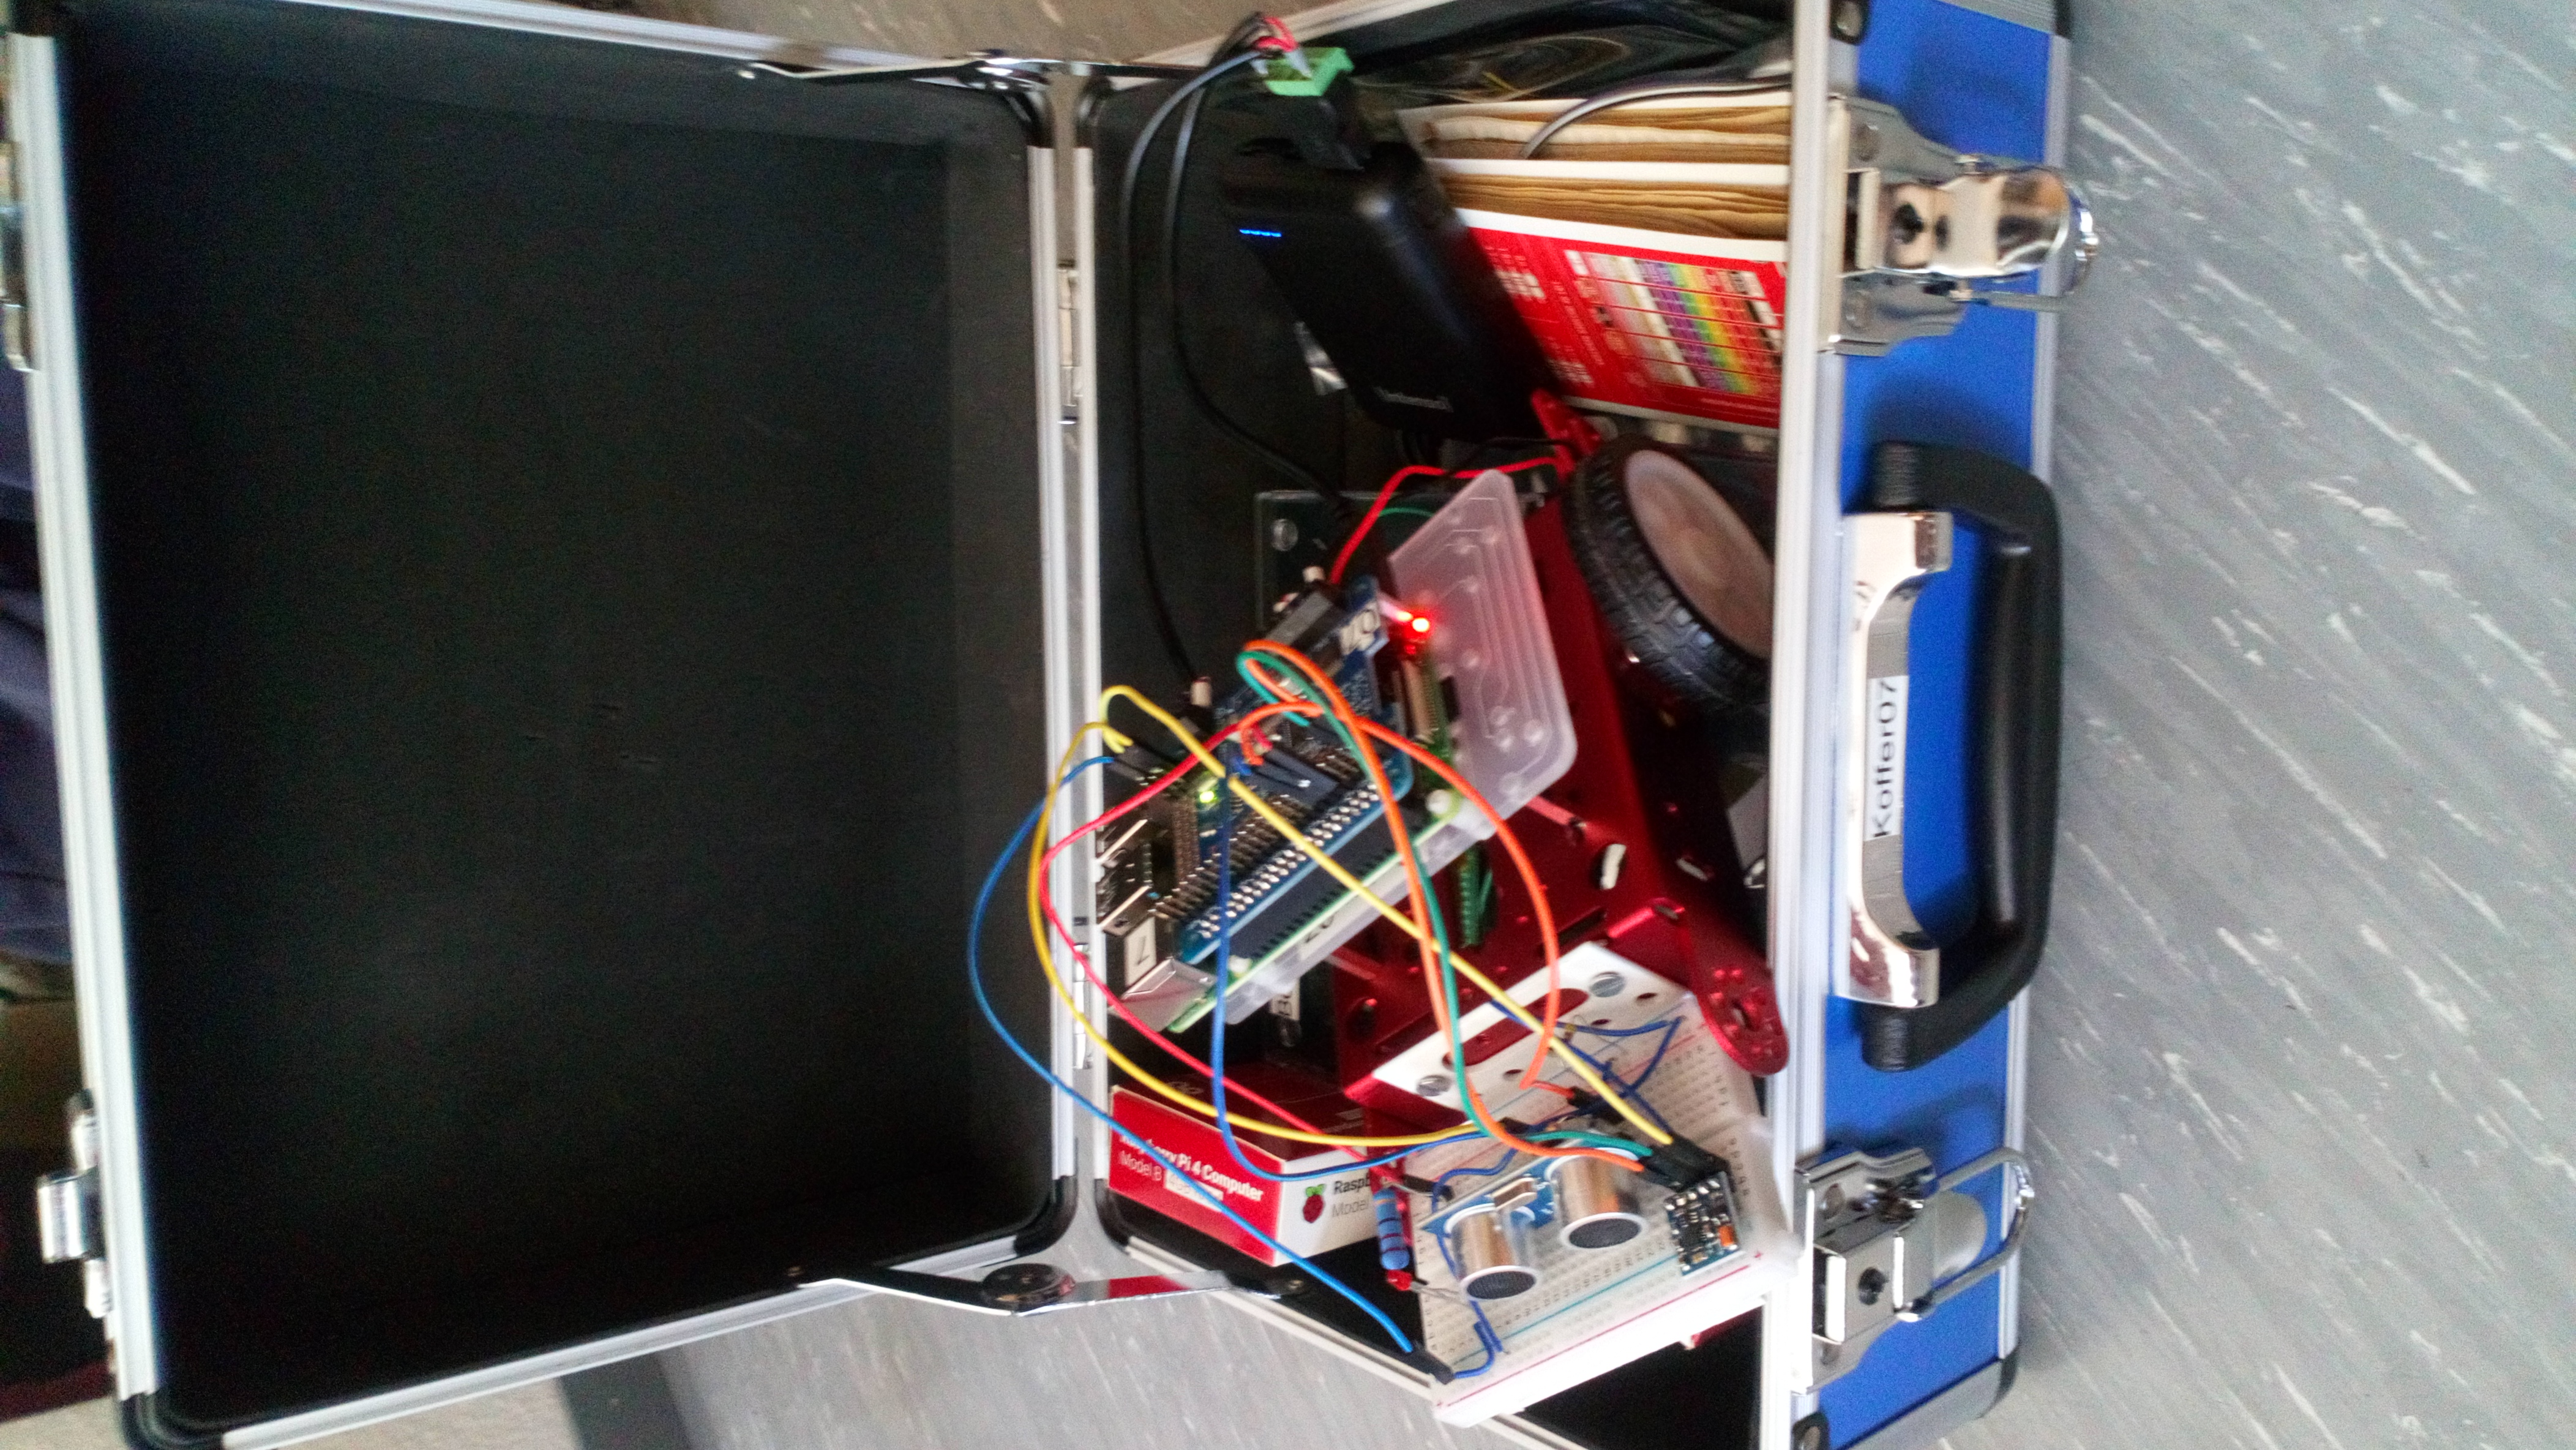
\includegraphics[width=0.45\linewidth, scale = 0.5]{lernportfolio_assets/BuggyZusammengebaut.JPG}
        \end{figure}
        \vspace{0.8cm}
        EES Buggy-Projekt 
        \pagebreak
    \end{center}
\end{titlepage}

\tableofcontents
\pagebreak

\begin{section}{Aufbau des Buggy}

\begin{figure}[h!]
  \centering
  \captionsetup[subfigure]{labelformat=empty}
  \begin{subfigure}{0.45\linewidth}
    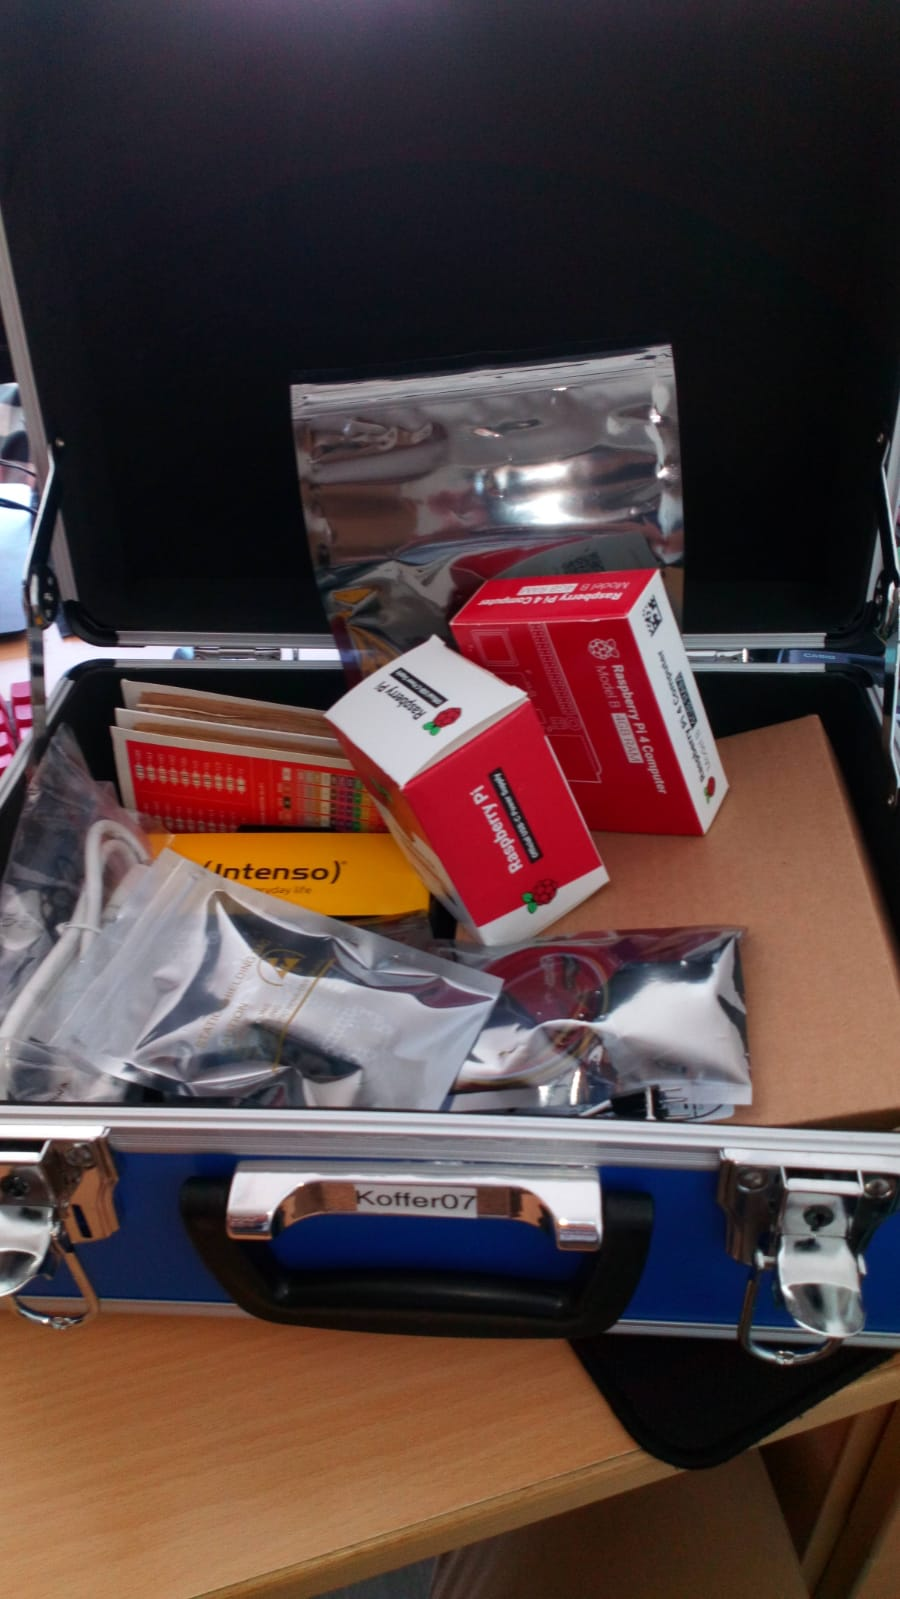
\includegraphics[width=\linewidth]{lernportfolio_assets/Buggy_Koffer.jpeg}
    \caption{Der Buggy vor dem Aufbau}
  \end{subfigure}
  \begin{subfigure}{0.45\linewidth}
    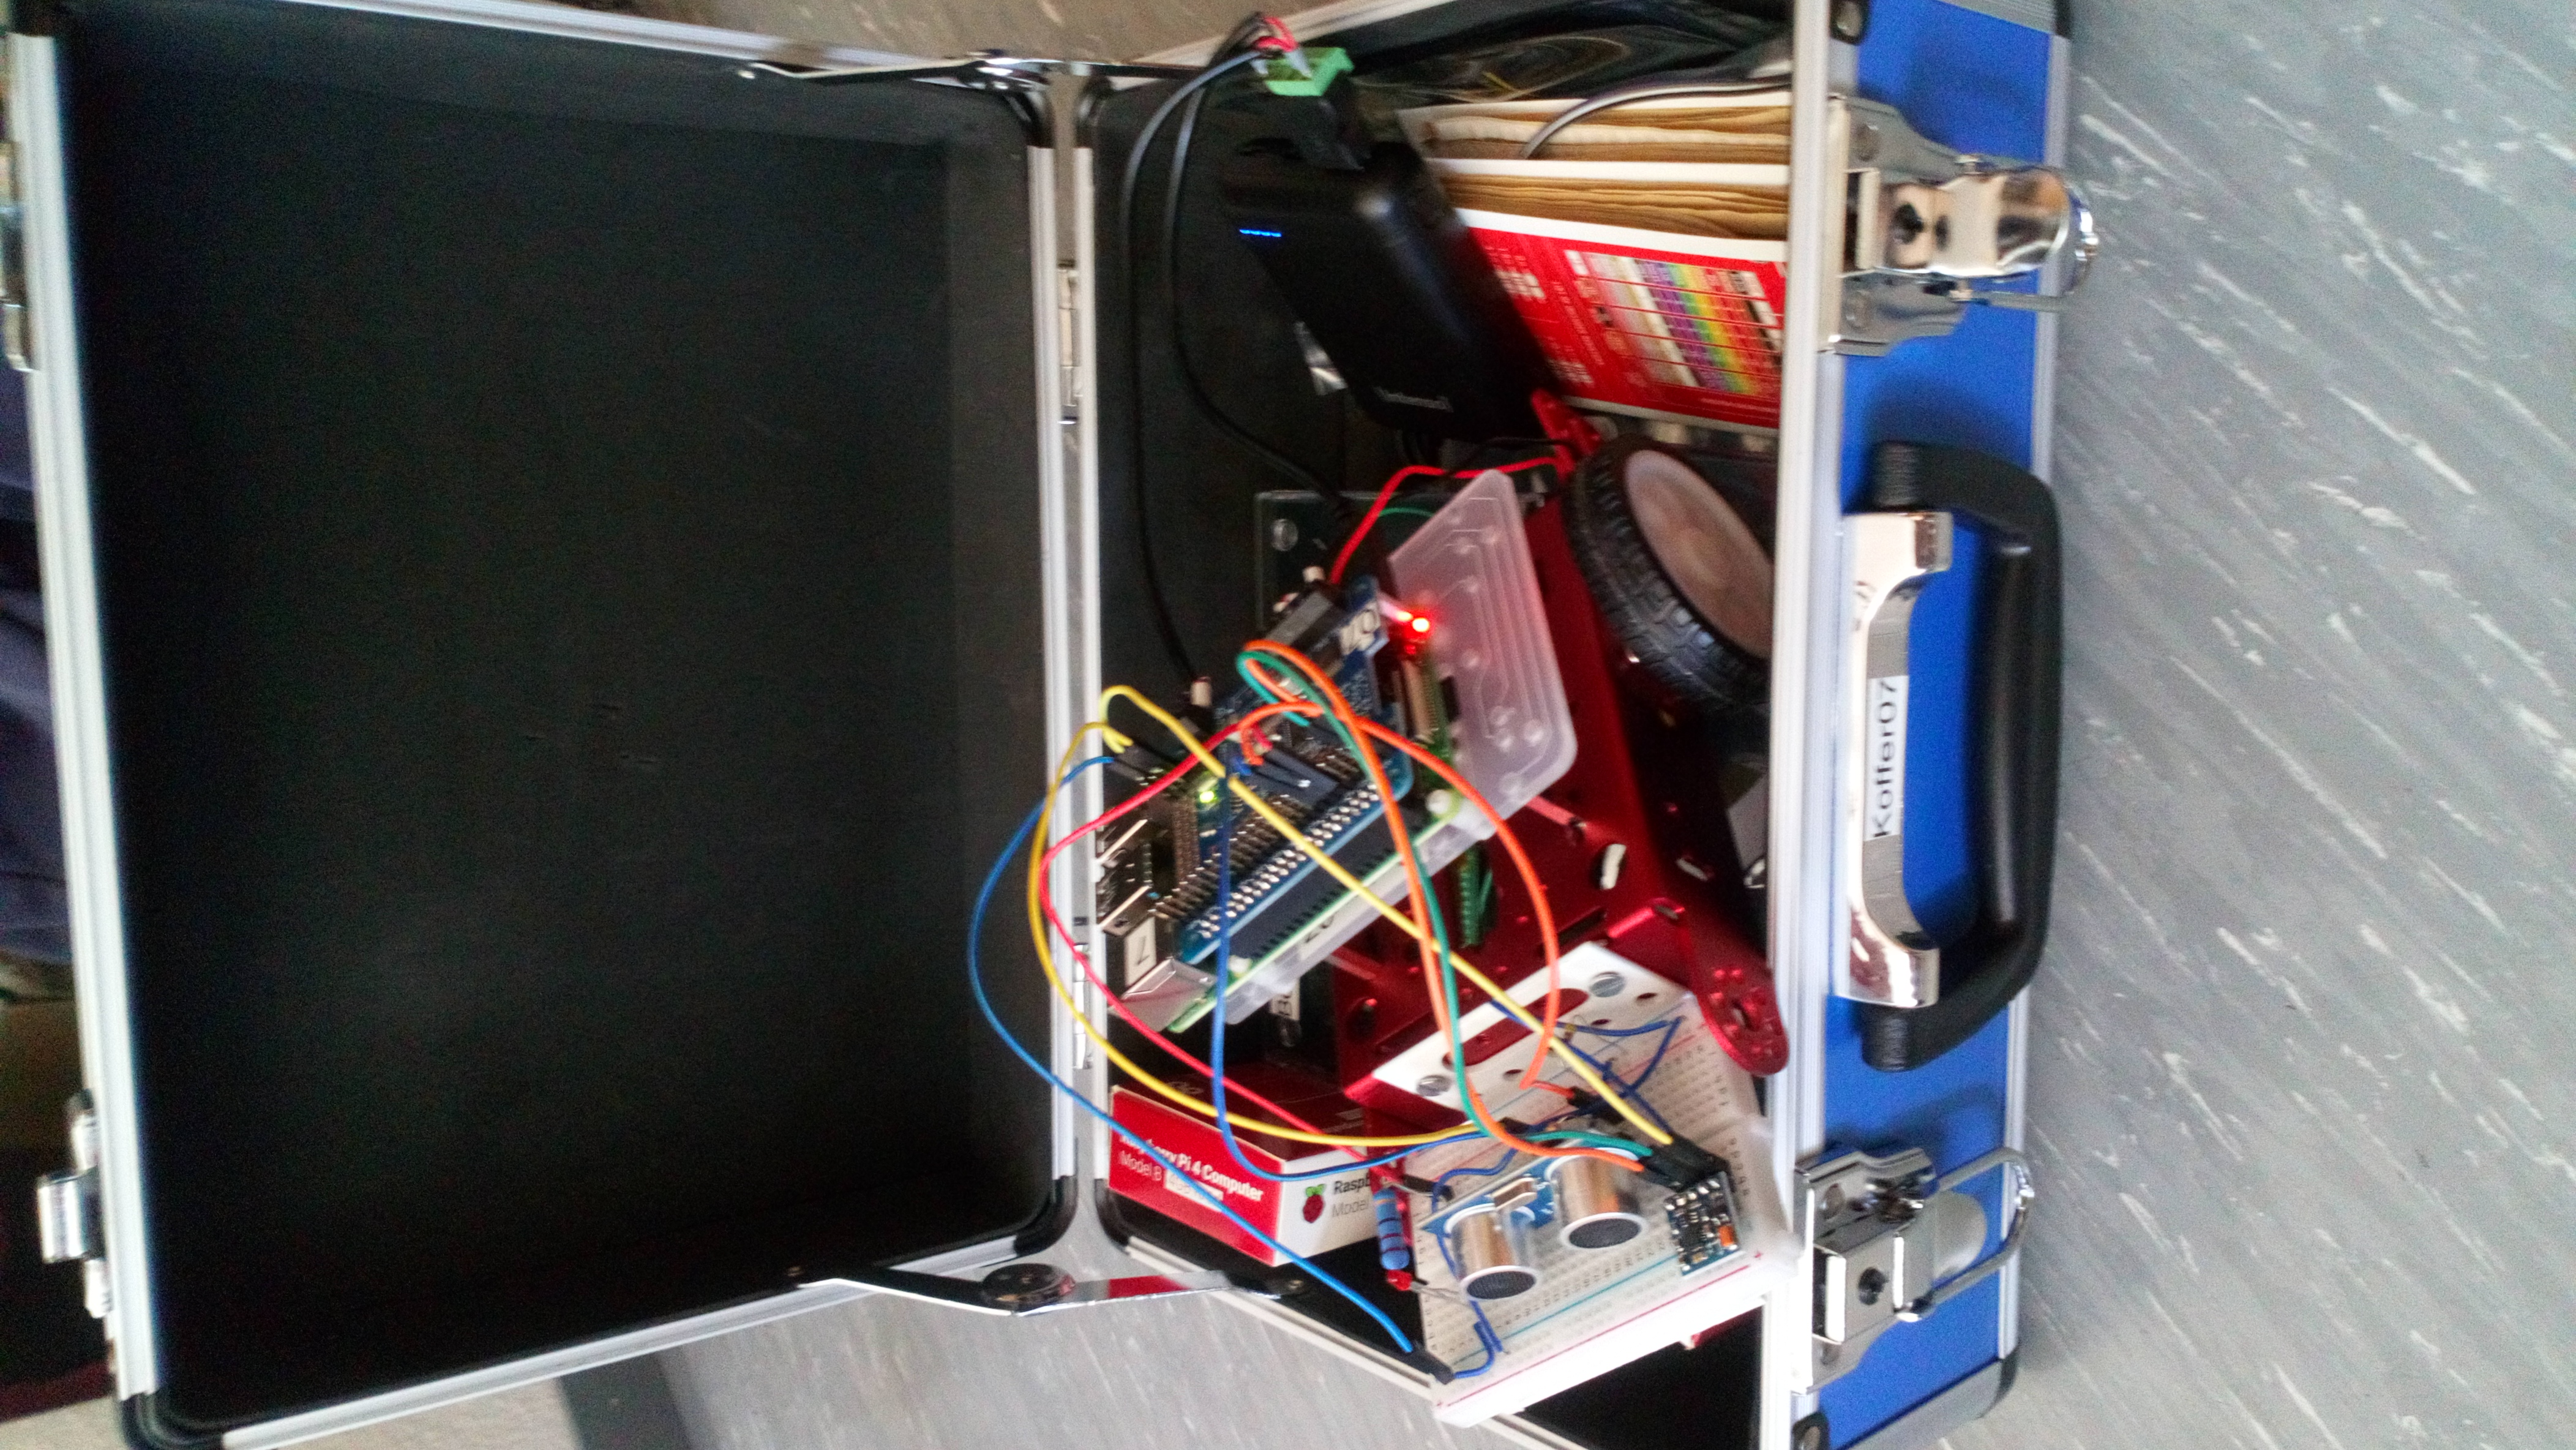
\includegraphics[width=\linewidth]{lernportfolio_assets/BuggyZusammengebaut.JPG}
    \caption{Und komplett aufgebaut}
  \end{subfigure}
\end{figure}

Der Buggy wurde vor der Herausgabe des Arbeitsauftrages zusammengebaut. Zwischenschritte sind daher nicht bildlich festgehalten. 

Der Zusammenbau des Buggys verlief problemlos. Der Text ist insgesamt verständlich geschrieben und war eine große Unterstützung.

% Wollen wir das aufnehmen?
% Im Text ist der Genetiv von "`der Buggy"' durchgehend "`des Buggies"'. Mit Verweis
% auf \url{https://www.duden.de/rechtschreibung/Buggy} ist der korrekte - und
% kontraintuitive - Genetiv "`des Buggys"'.
In den meisten Bildern (außer auf Seite IV) ist der Buggy mit roter Platte gezeigt, wenngleich die Anleitung hier den weißen Winkel vorsieht. Eine Anmerkung, dass der Buggy im Folgendem mit roter Platte statt Winkel gezeigt wird, hätte eine kurze Verwirrung meinerseits verhindert.

Als Ubuntu-Nutzer bzw. Linux-Nutzer muss man keine zusätzliche Software installieren um eine SSH-Verbindung herzustellen. Eine Ergänzung, dass \href{https://invisible-island.net/xterm/}{XTerm} eine Empfehlung an die Windows-Nutzer ist, wäre daher angebracht. Bei dieser Bemerkung wird davon ausgegangen, dass mit XTerm an dieser Stelle \href{https://mobaxterm.mobatek.net/}{MobaXterm} gemeint ist und nicht der Terminal Emulator XTerm. 

Für den kompletten Zusammenbau wurden insgesamt 1,5 Stunden benötigt.

%Das meinst du nicht ernst oder ??? Ich bin dafür das kommt raus.
% Das ist der Punkt 1.4 aus  Arbeitsauftrag Projektphase_EES.pdf? 
Weil der Buggy schon vor Herausgabe des Arbeitsauftrages und während der anhaltenden Corona Phase abgeholt worden ist, wurde der Buggy von einer Person aufgebaut. Im Nachhinein haben wir uns trotzdem Gedanken dazu gemacht, wie wir den Aufbau am besten hätten aufteilen können. Wir sind zu dem Ergebnis gekommen, dass jede Person einen Teil des Buggys aufbauen sollte. Konkret hätte sich einer um das Kugellager und die Motoren gekümmert. Einer um die Abstandhalter und das Anbringen der Plastikplatte und des Raspberry Pi. Der letzte um das Anbringen des Motorhats und um das Anschließen und Fixieren der Powerbank.

\end{section}

\begin{section}{Motorensteuerung}
  Die Aufgabenstellung wurde so verstanden, dass man die Motorensteuerung
  selbst implementieren sollte. Das Lösen der Aufgabe geschah vor Erscheinen des
  erklärenden Forenposts. Daher wird im Folgendem auch über das Erstellen des
  Motorentreibers reflektiert.

  Herausforderungen bei der Programmierung waren vor allem 4 Punkte: 1. Finden der wichtigen
  Dokumentation, 2. Verstehen der Dokumentation, 3. Extraktion der relevanten
  Informationen und 4. Analyse des Beispielcodes.

  Der Motorhat ist mit dem RaspberryPi über \itoc{} verbunden. Die
  \wiringPi{}\cite{wiringPi} Bibliothek ermöglicht das Verbinden, Schreiben und Lesen von
  Registern über dieses Protokoll auf komfortablem und leicht verständlichem Wege.
  Bei der Benutzung dieser Bibliothek kam es zu keinen Problemen.
  
  Durch die Schematas \cite{motorhatDownloads}
  konnte die Verknüpfung der Pins des PCA9685 PWM LED Controllers mit den beiden
  TB6612FNG Motorsteuerungschips nachvollzogen werden.
  Durch die Datenblätter \cite{datasheetPCA9685} und \cite{datasheetTB6612}
  wurde die Funktionsweise des Referenzcodes \cite{referenzcode}
  verständlich, wenngleich hierbei eine Frage offengeblieben ist:
  Der Referenzcode schreibt den Wert 4096 in ein LED On bzw. Off Register um den
  jeweiligen Motor an bzw. auszuschalten. In der Dokumentation des PCA9685 PWM LED
  Controllers heißt es jedoch unter Punkt 7.3.4 : "`The LEDn\_ON and LEDn\_OFF
  counts can vary from 0 to 4095"'.

  In den ersten Testläufen hat sich der Buggy beim Forwärtsfahren im Kreis
  gedreht. Die Motoren haben in unterschiedliche Richtungen gedreht. Dieses
  Verhalten war richtig, da beide Motoren auf forwärts gestellt waren, was
  synonym für eine rechtsläufige Bewegung ist. Für das rechte Rad bedeutet
  rechtsläufig forwärts. Für das linke Rad, welches durch den Anbau 
  \ang{180} um die Z-Achse gedreht ist, bedeutet dies rückwärts.
  Das Problem konnte behoben werden, indem die beiden Pins, welche für die Richtung
  zuständig sind, vertauscht wurden. So wurde jede rechtsläufige Bewegung zu einer
  linksläufigen und vice versa. Ein Forwärts-Kommando an das linke Rad wurde nun
  korrekterweise automatisch in eine linksläufige Bewegung übersetzt.
  Weiterhin war es ein Problem den Buggy konsistent losfahren zu lassen. Niedrige 
  Geschwindigkeit sind beim Start zu gering, um die Motoren drehen zu
  lassen. Das hat dazu geführt, dass der Buggy oft nicht losfuhr, trotz eines
  forwärts Kommandos. Dieses Problem konnte behoben werden, indem eine Mindestgeschwindigkeit
  eingestellt worden ist, sodass der Buggy nicht mit niedrigen Geschwindigkeiten
  konfigurierbar ist.

  Neben den technischen Herausforderungen war auch das Testen des Codes auf dem
  Raspberry Pi eine Umgewöhnung. Der Code konnte nicht lokal (auf dem eigenen
  Rechner) getestet werden, da die \wiringPi{} Bibliothek nur auf einem Raspberry Pi funktioniert.
  Als Workflow hat sich durchgesetzt, dass auf dem eigenen Rechner entwickelt
  wurde, die Änderungen commitet und in das \githubrepo{} gepusht worden sind.
  Danach wurde der neue Code auf dem Raspberry Pi runtergeladen, die Binary
  durch "`cmake . \&\& make"' gebaut und schließlich getestet. Kleine Änderungen
  wurden auf dem Raspberry Pi durch den Texteditor Vim vollzogen.

  Besonders hilfreich war zur Lösung dieser Aufgabe, die Vertrautheit im Umgang
  mit Datenblättern, die man aus der Vorlesung bzw. Praktikum mitgenommen hat.
  Das Verstehen der Registertabellen fiel deutlich einfacher als beim ersten
  mal und das Unterscheiden zwischen wichtigen und unwichtigen Informationen
  ging schneller.


  Videos auf denen der Buggy geradeaus, slalom und verschiedene andere
  Bewegungen ausführt, können im Video Ordner eingesehen werden.
  Hierbei ist auffällig, dass der Buggy dazu neigt, bei gerader Fahrt nach links
  abzudriften.

  Zur manuellen Steuerung des Buggys wurde ein
  \href{https://invisible-island.net/ncurses/announce.html}{ncurses} basiertes
  Benutzerinterface gebaut. Die Steuerung funktioniert über die Tasten W, A, S
  und D. Q kann für zur Durchführung eines langsamen Stopps und E zur
  Durchführung eines schnellen Stopps betätigt werden. Durch X wird das
  Benutzerinterface geschlossen.
  In dem Interface werden im oberem Bereich die aktuellen Sensordaten angezeigt.

  \begin{figure}[h!]
    \centering
    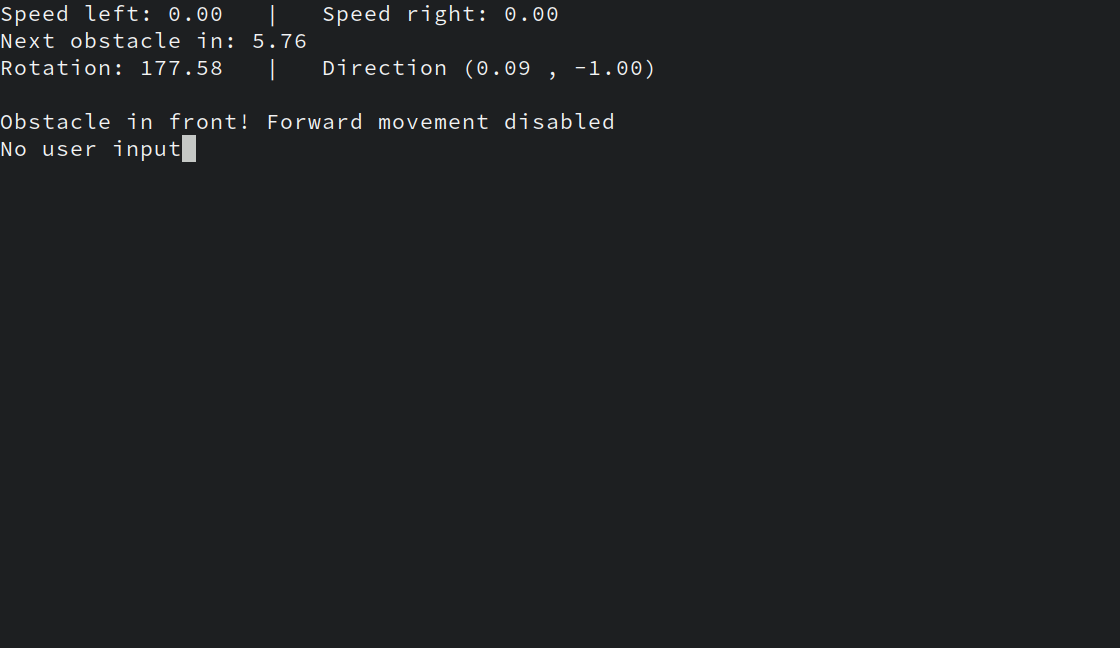
\includegraphics[width=0.75\textwidth]{lernportfolio_assets/WasdBenutzerinterface.png}
    \caption{Benutzerinterface für die manuelle Steuerung des Buggys}
  \end{figure}

\end{section}

\begin{section}{Ultraschallsteuerung}
    % START task 3.1 of Arbeitsauftrag Projektphase_EES.pdf
    \begin{subsection}{Recherche zum Ultraschallsensor und der Entfernungsmessung}
        Bei der Suche nach einem Datasheet zum HC-SR04 haben wir vergeblich nach
        einem offiziellen Datasheet gesucht. Daher haben wir uns  verschiedene 
        Datasheets \cite{datasheetUltrasonic1,datasheetUltrasonic2,
          datasheetUltrasonic3} zum HC-SR04 angeschaut und die Spezifikationen gründlich
        miteinander verglichen um sicher zu gehen, dass die Werte stimmen.
        Um auf eine Formel für die Distanzberechnung mithilfe von Ultraschall
        zu kommen haben wir nach der Geschwindigkeit von Schall in Luft gesucht.
        Dadurch können wir nun mit Hilfe des Sensors die Distanz des Buggys zum
        nächsten Objekt mit folgender Formel berechnen:\\
        Distanz in \si\cm = \( \frac{Signalzeit}{2} \) \si{\milli\second} $ \times $ 34.3 \si[per-mode = fraction]{\cm\per\milli\second}
    \end{subsection}
    % END task 3.1

    % START task 3.3 of Arbeitsauftrag Projektphase_EES.pdf
    \begin{subsection}{Steuerung und Auslesen von GPIOs}
        % Was haben Sie über die Steuerung und Auslesen von GPIOs gelernt
        % und welches Wissen und Techniken aus dem ersten Teil der Vorlesung
        % konnten Sie einsetzen?
      %PRAISE THE LORD IN HIS ALMIGHTY. AMEN
        Dank der Vorlesung haben wir gelernt, dass die GPIO Pins verschiedene
        Modi besitzen. Um Signale zu senden muss man sie in den Output-Mode 
        versetzen. Wenn man Signale empfangen will muss man den Pin in
        den Input-Mode versetzten. Hier haben wir gelernt wie wichtig es ist 
        auch die korrekte Spannung angelegt zu haben! Sowohl beim STM32 als auch
        beim Raspberry Pi darf die Eingangsspannung 3.3V nicht überschreiten.
        Höhere Eingangsspannungen (wie etwa die 5V die vom Ultraschallsensor 
        ausgehen) können das Gerät zerstören! Wir haben ebenfalls gelernt, 
        dass es zu einem floating State kommen kann, wenn wir keine Pull-up 
        bzw. Pull-down Widerstände einsetzen. Dies kann bei der 
        Nachimplementierung für bestimmte Protokolle genutzt werden. Bei unserem
        Anwendungsfall gilt es jedoch, diese zu verhindern und klare Low und High
        Pegel zu erhalten.\\
        Mit unseren Kenntnissen konnten wir nun einen Schaltplan anfertigen:
        % testing figure
        \begin{figure}[H]
        \centering
            \begin{minipage}{0.49\textwidth}
                \centering
                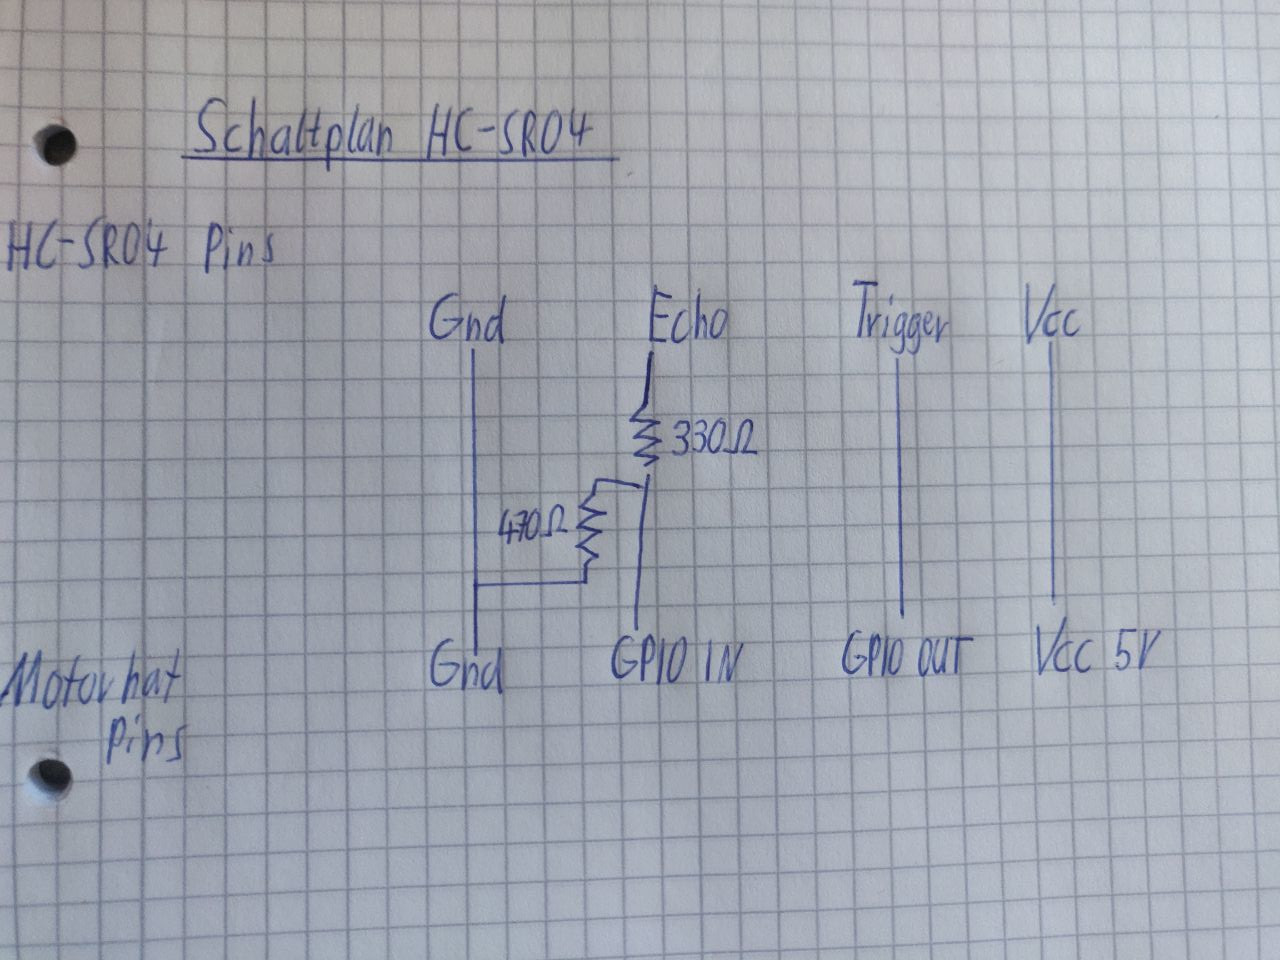
\includegraphics[width=0.9\textwidth]{lernportfolio_assets/UltraschallsensorSchaltplanAufPapier.jpg}
                \caption{Auf Papier geplant}
            \end{minipage}
            \centering
            \begin{minipage}{0.49\textwidth}
                \centering
                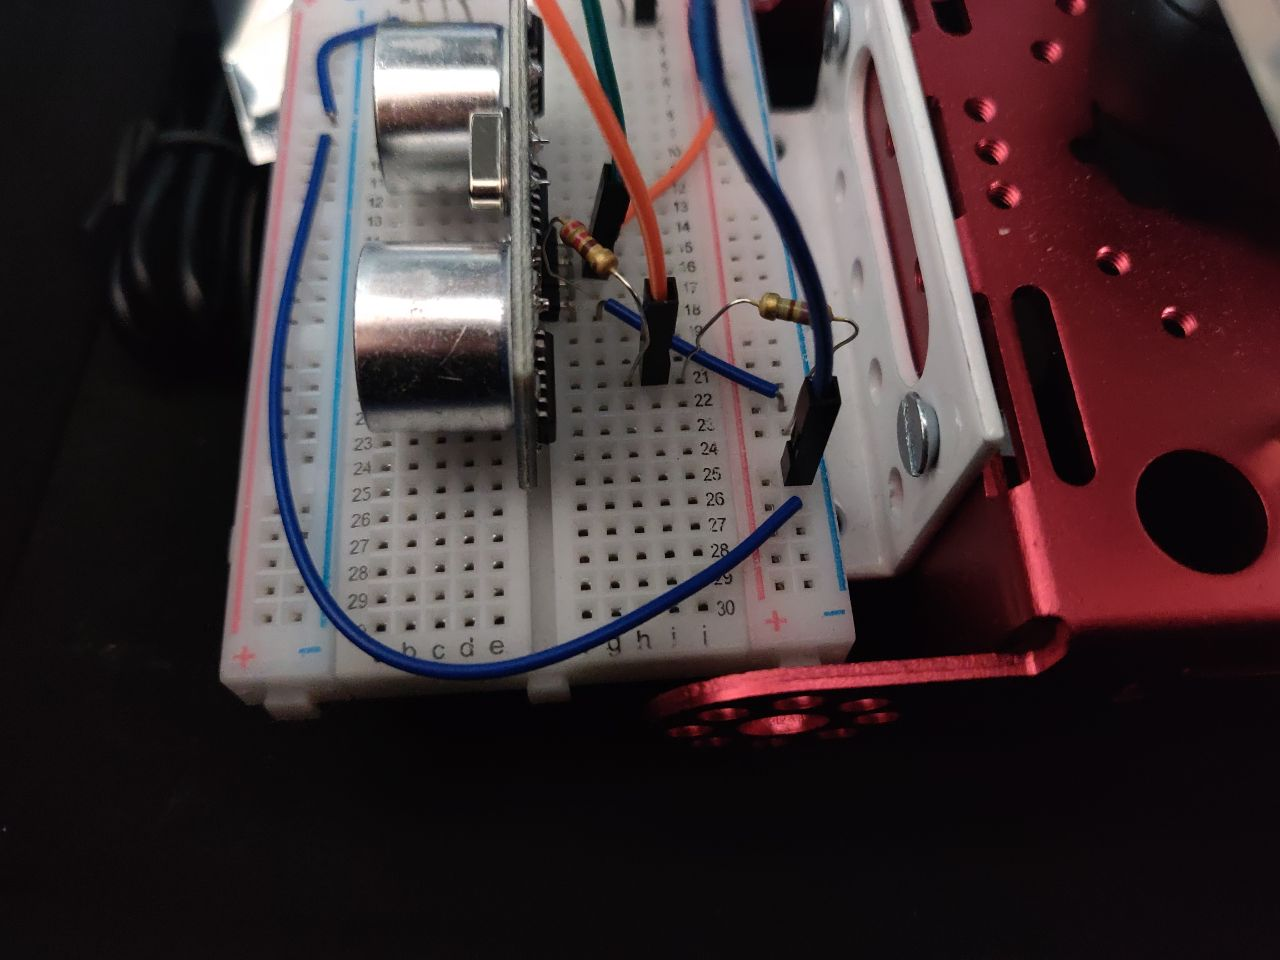
\includegraphics[width=0.9\textwidth]{lernportfolio_assets/UltraschallsensorSchaltplanImBuggyVerbaut.jpg}
                \caption{Im Buggy verbaut}
            \end{minipage}
        \end{figure}

    \end{subsection}
    % END task 3.3

    % START task 3.4 of Arbeitsauftrag Projektphase_EES.pdf
    \begin{subsection}{Stolpersteine bei der Programmierung}
        % Erörtern Sie, was bei der Programmierung der Entfernungsmessung
        % mit dem Ultraschallsensor besonders wichtig ist.
        Durch das Einbinden des Ultraschallsensors in unser Program sind wir auf
        einige Fehlerquellen gestoßen. Im folgenden erläutern wir die Lösunen zu
        unseren Problemen.
        \begin{paragraphwithnewline}{Theorie und Praxis}
            Laut Datenblatt muss der Trigger pin für mindestens 10 \si{\micro\second}
            auf High gesetzt werden um die Ultraschallwelle auszulösen. Dadurch
            hat man bei manchen Messungen jedoch kein Signal beim Trigger erzeugt
            und hat dadurch komplett falsche Werte erhalten. Hier hat sich
            schnell gezeigt, dass es in der Praxis besser ist eine gewisse Fehlertoleranz
            einzubauen. Den Wert auf 20\si{\micro\second} zu erhöhen hat unser
            Problem dann gelöst.
        \end{paragraphwithnewline}

        \begin{paragraphwithnewline}{Falsche Messwerte filtern}
            Durch Störungen wird der Ultraschallsensor auch ggfs. falsche Werte
            erzeugen. Um das Messergebnis nicht zu verfälschen muss man einen
            Mechanismus einfügen der überprüft, ob die erhaltenen Werte wirklich
            sinnvoll sind. 
        \end{paragraphwithnewline}

        \begin{paragraphwithnewline}{Distanz möglichst genau berechnen}
            Die Messvarianz kann bei einzelnen Messungen das Ergebnis stark
            beeinflussen. Um dem entgegenzuwirken wird die Messung mehrmals
            wiederholt und die Distanz auf Basis des Mittelwerts gebildet.
        \end{paragraphwithnewline}


    \end{subsection}
    % END task 3.4

    % START task 3.5 of Arbeitsauftrag Projektphase_EES.pdf
    \begin{subsection}{Bewertung der Zuverlässigkeit der Entfernungsmessung}
      Die Entfernungsmessung funktioniert für solide Objekte in einer Reichweite
      von 5 bis 100 cm zuverlässig. Für weniger solide Objekten, wie z.B. einer
      Pappierbox, hat der Sensor bei den Tests Probleme
      gehabt, die Entfernung richtig einzuschätzen. Oftmals kam es hierbei zu keinen Rückmeldungen an den Echo-Pin. Dieses
      Problem wurde durch ein Zeitlimit beim Warten auf den Echo-Pin gelöst und
      verwerfen der Messung falls das Zeitlimit überschritten wurde. Das
      Ermitteln der Entfernung beinhaltet mehrere Entfernungsmessungen. Somit
      ist das verwerfen einzelner Messungen durch ein überschreiten des
      Zeitlimits vertretbar. Aus den Messungen wird anschließend ein Mittelwert
      gebildet und zurückgegeben. Durch mehrmaliges Messen und bilden des
      Mittelwertes wird zugleich die relativ hohe Varianz zwischen einzelnen
      Messungen bei gleicher Distanz zum Objekt abgefangen.
    \end{subsection}
    \begin{subsection}{Bewertung der Genauigkeit}
      Die Entfernungsmessung funktioniert mit einer Standardabweichung von unter
      1,3 cm auf 100 cm genau.
      Die Rohdaten können im Ordner
      \gquotes{test\_data\_ultrasonic} eingesehen werden.
      Im folgendem eine Zusammenfassung.
      %The table is generated by pandas
      \begin{table}[h!]
        \begin{tabularx}{\textwidth}{XXXXXXXX}
            {} &     5cm &    10cm &    15cm &    20cm &    30cm &    50cm &   100cm \\
            count &  100.00 &  100.00 &  100.00 &  100.00 &  100.00 &  100.00 &  100.00 \\
            mean  &    4.67 &    9.36 &   13.95 &   19.94 &   30.42 &   51.08 &   99.55 \\
            std   &    0.03 &    0.31 &    0.11 &    0.06 &    0.11 &    0.48 &    1.27 \\
            min   &    4.65 &    8.79 &   13.80 &   19.81 &   30.08 &   50.05 &   91.35 \\
            25\%   &    4.66 &    9.12 &   13.85 &   19.88 &   30.41 &   50.82 &   99.67 \\
            50\%   &    4.66 &    9.31 &   13.91 &   19.93 &   30.45 &   51.00 &   99.88 \\
            75\%   &    4.67 &    9.66 &   14.02 &   19.98 &   30.48 &   51.52 &   99.96 \\
            max   &    4.98 &    9.82 &   14.23 &   20.13 &   30.57 &   51.95 &  100.91 \\
          \end{tabularx}
        \caption{Zusammenfassung der Rohdaten. Alle Werte in cm.}
    \end{table}
    Aus der Tabelle geht hervor, dass der Abstand zu nahen
    Objekten (Abstand $\leq{} 20 cm$) tendenziell unterschätzt wird, zu entfernteren
    Objekten hingegen geringfügig überschätzt. Eine Ausnahme bildet hier die
    Messreihe für den Abstand von 100 cm.
    
    Um den Mittelwert gibt es für alle Werte eine Standardabweichung von weniger
    als 1,3 cm. Die Messungen sind daher präzise. Erwähnenswert ist, dass die
    Standardabweichung bei kleineren Distanzen sehr viel geringer ist als bei größeren.

    \begin{figure}[H]
      \centering
      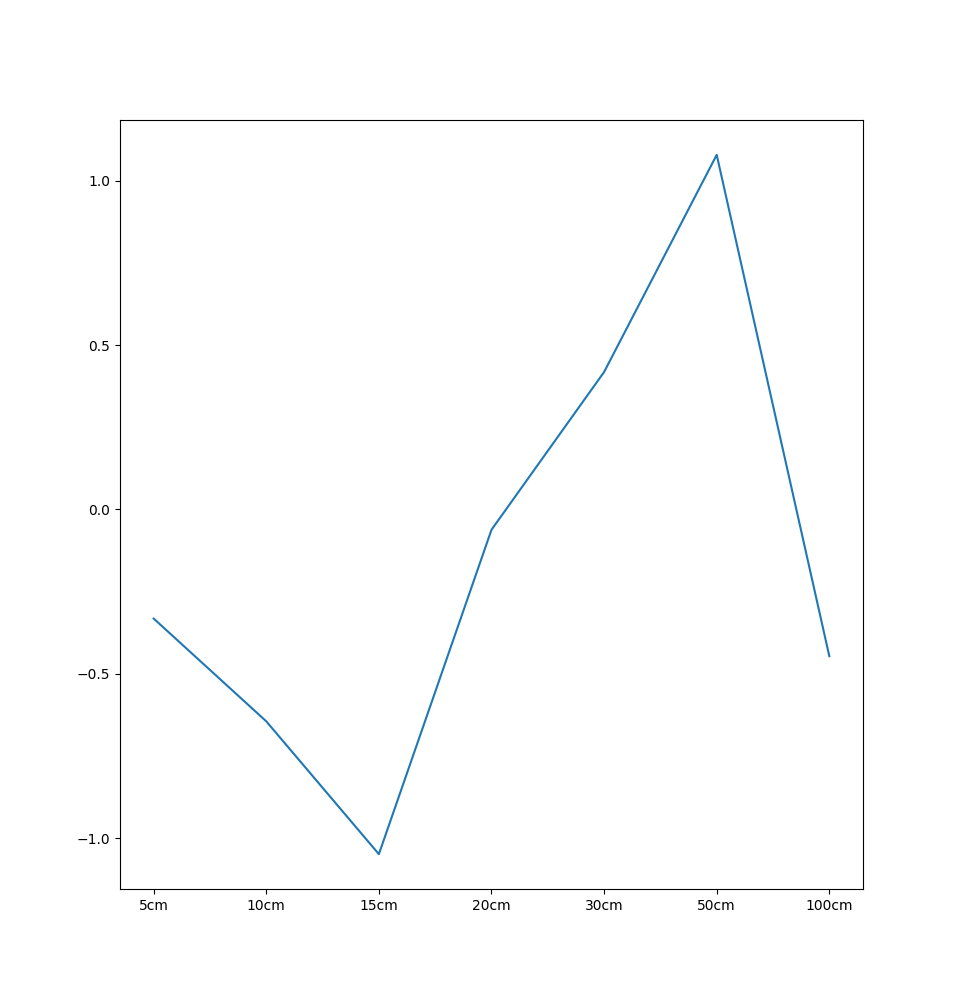
\includegraphics[width=0.5\textwidth]{test_data_ultrasonic/meanDiff.png}
      \caption{Differenz des Mittelwertes zur tatsächlichen Distanz}
    \end{figure}

  \end{subsection}
  \begin{subsection}{Integration in das Programm}
    Kommt der Buggy unter manueller Steuerung via des Benutzerinterfaces oder
    automatischer Steuerung durch die Klasse "`automatic\_movement"' zu nah
    an ein Gegenstand, hält der Buggy an. Bei der manuellen Steuerung geht zusätzlich
    das "`Bremslicht an"'.
    Das Anhalten ist in dem Video "`NothaltVorWand.mp4"' dargestellt.
  \end{subsection}
  % END task 3.5

\end{section}

\begin{section}{Kompass}
  \begin{subsection}{Relevante Informationen aus dem Datenblatt}
    Aus dem Datenblatt \cite{datasheetMagnet} konnte die korrekte Verkabelung
    entnommen werden.

  Im Datenblatt stößt man als erstes auf die \itoc{} Adresse des Kompass, mit der man dann z.B. mit dem Befehl 
  "`i2cdetect -y 1"' überprüfen kann, ob der Kompass richtig angeschlossen ist. Die Adresse des Kompass ist "`0x0D"' 
  und wurde in der Tabelle der \itoc{} Geräte angezeigt.
  
  Die nächsten relevanten Informationen sind Anwendungsbeispiele. Hier sieht man schnell, welche Register für 
  uns besonders relevant werden. Darunter: das Set/Reset-Register 0BH, das
  Control-Register 09H, das Statusregister 06H und die Datenregister 00H bis 05H. 
  
  Wenn man dem Beispiel folgt und sich die Register anguckt, wird hier das Set/Reset-Register auf 0x01 gesetzt.
  Bei den Informationen zu dem Register wird nur empfohlen das Register auf den genannten Wert 0x01 zusetzen. 
  Weitere Informationen zum Set/Reset-Register werden nicht genannt.
  
  Danach kommt das Control Register. Hier werden die gewünschten Einstellungen für den Kompass in zwei Bit 
  Abfolgen gesetzt. Als erstes der Modus. 0x00 steht für Standby und 0x01 für
  Continous. Danach kommt die "`Output Data Rate"', kurz ODR, 
  also die Rate in der beim Continous Modus neue Daten in die Datenregister
  geschrieben werden. Danach folgt RNG für die 
  Sensitivität des Kompass, welches in 2 oder 8 Gauss gemessen wird. Zuletzt
  kommt die "`Over sample Rate"', kurz OSR, für die Bandbreite eines internen digitalen Filters.
  
  Als letztes kommen die Datenregister und ein Statusregister. Das Statusregister hat drei Bits. Davon ist für 
  uns überwiegend das erste - das DRDY Bit - relevant. Das DRDY Bit wird vom Kompass auf 1 gesetzt, sobald neue Daten 
  geschrieben werden.
  \end{subsection}
  \begin{subsection}{Erstes Programmieren des Treibers}
  Für den Treiber konnten wir die \wiringPi{} Bibliothek wiringPiI2C benutzen, die wir bereits in der 
  Implementierung des Motorhat-Treibers benutzt hatten. Der Treiber wird durch
  die Klasse \gquotes{magnetic\_sensor} repräsentiert. Für das Setup des Treibers wird der Konstruktor benutzt. 
  Der Standardkonstruktor initialisiert den Kompass auf die Beispieldaten vom Datenblatt.
  
  Um die ersten Daten zu bekommen haben wir hier eine check() Methode benutzt. Damit können wir neben dem
  einfachen Einlesen der Datenregister vom DRDY Bit einen Vorteil ziehen. Wenn dieses gesetzt ist, müssen wir 
  keine neuen Daten einlesen, da die alten Daten noch aktuell sind. Wenn das Bit für längere Zeit auf Null bleibt
  wissen wir so auch, dass etwas beim Setup fehlgeschlagen ist.
  %TODO @Jens Dieser Halbsatz macht für mich keinen Sinn. Warum ist das Setup
  %fehlgeschhlagen wenn man check aufruft ohne dass das DRDY Bit gesetzt ist?
  %%% und wir wissen schneller ob nicht etwas beim Setup fehlgeschlagen ist. %added
  Falls die Daten aktualisiert worden sind, gibt die Methode eine Eins zurück. Ansonsten eine Null. 

  Nachdem wir nun die ersten Register gelesen hatten und wussten, dass der Kompass funktioniert, mussten wir nun die Daten 
  zusammensetzten. Die 16 Bit Daten für die Achsen sind nämlich immer jeweils in zwei 8 Bit Registern gesetzt. Ein 
  %TODO @Jens hier doch eher least/most significatn byte
  LSB (least significant byte) und ein MSB (most significant byte).
  
  Beim recherchieren zum Kombinieren der Daten stoßten wir auch auf einen Forumsbeitrag\cite{forumMagnet}
  bei dem man den Vorteil von C++ für diese Aufgabe sehen konnte. Genauer genommen die 
  Möglichkeit Variablen als signed 16-Bit-Integer zu deklarieren. Dadurch konnten wir die Daten kombinieren, ohne 
  groß weiter auf das Komplement einzugehen, was z.B. in Python nicht so leicht ist.
  \end{subsection}
  \begin{subsection}{Genauigkeiten der Daten und Sensitivität}
  Die Rohdaten können im Ordner \gquotes{test\_data\_magnetic\_sensor} eingesehen werden.
  Beim ersten Drehen des Buggys zum analysieren der Kompassdaten, gab es eine stärkere Störungsstelle und man 
  konnte schnell sehen, wie sensibel der Kompass ist. Die Störung konnte man dann auch mit einem normalen Kompass 
  ausfindig machen.
  Eine zweite Messreihe wurde in einem anderen Raum durchgeführt.

  \begin{figure}[h!]
    \centering
    \captionsetup[subfigure]{labelformat=empty}
    \begin{subfigure}{0.45\linewidth}
      \centering
      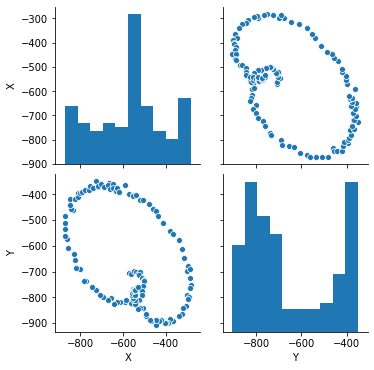
\includegraphics[width=\linewidth]{lernportfolio_assets/MagnetDatenStorung}
      \caption{Messungen mit Störung}
    \end{subfigure}
    \begin{subfigure}{0.45\linewidth}
      \centering
      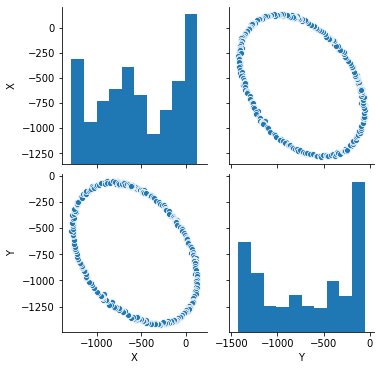
\includegraphics[width=\linewidth]{lernportfolio_assets/MagnetDaten}
      \caption{Messungen ohne Störung}
    \end{subfigure}
  \end{figure}
  
  Jetzt kann man sehen, dass die Werte eine Ellipse darstellen. Da der Sensor im
  Kreis gedreht worden ist, war zu erwarten, dass die Werte in Kreisform
  angeordnet sein werden. Auch bei Wiederholung der Messung gab der Sensor Daten
  in Ellipsenform aus. Daher handelt es sich hierbei aller Wahrscheinlichkeit
  nach um eine Fehlfunktion. Denn durch die Ellipsenform werden die
  y-Koordinaten im Bezug zu den x-Koordinaten überschätzt.

  Dieses ist jedoch korrigierbar. Eine Ellipse kann in einen Kreis transformiert
  werden, indem der Ursprung der Ellipse nach (0, 0) verschoben wird, die
  Ellipse gedreht wird, bis sie Achsensymetrisch ist und anschließend die
  x-Koordinaten gestreckt werden.

  \begin{figure}[h!]
    \centering
    \captionsetup{justification=centering}
    \captionsetup[subfigure]{labelformat=empty}
    \begin{subfigure}{0.45\linewidth}
      \centering
      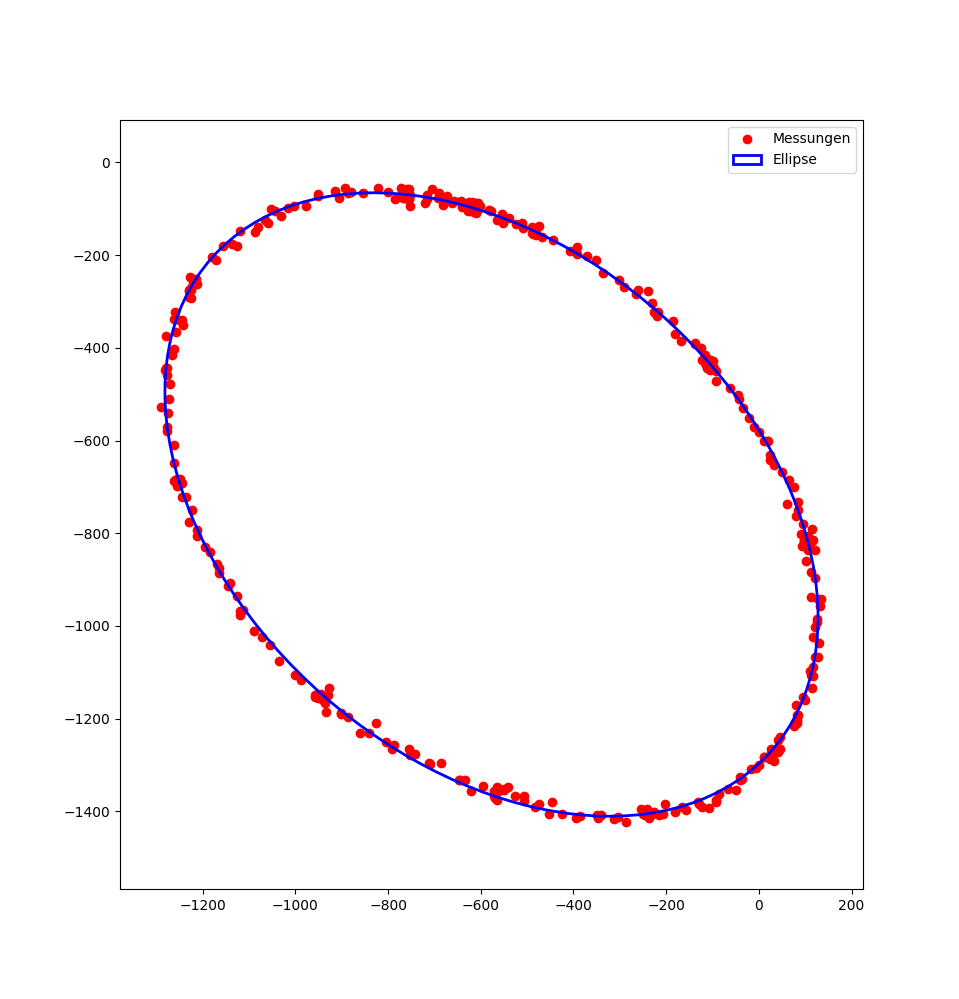
\includegraphics[width=\linewidth]{lernportfolio_assets/MagnetDatenMitEllipse.png}
      \caption{Daten vor der Transformation}
    \end{subfigure}
    \begin{subfigure}{0.45\linewidth}
      \centering
      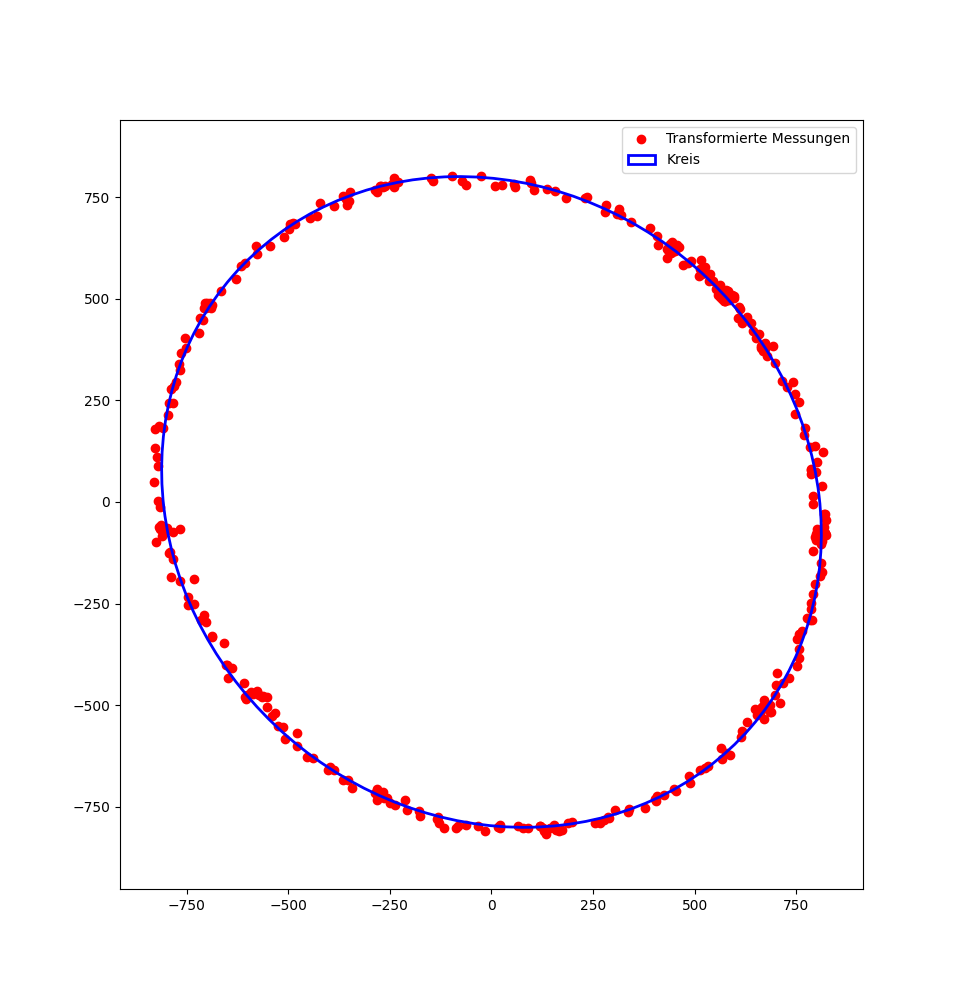
\includegraphics[width=\linewidth]{lernportfolio_assets/MagnetDatenAlsKreis.png}
      \caption{Daten nach der Transformation}
    \end{subfigure}
  \end{figure}
  
  Nach der Kalibrierung schwankten die Daten zu stark, um darauf basierend
  Entscheidungen beim Fahren zu treffen. Häufig kam es zu Ausreißern. Daher kam
  es zur Implementation der Klasse "`Compass"'. Diese Klasse fragt den
  Magnetsensor zyklisch nach neuen Daten ab und ermittelt basierend auf den
  Daten einen gleitenden Mittelwert, wobei die neuesten Messwerte mit fünf facher
  Gewichtung in die Rechnung eingehen, um der Phasenverschiebung auf Kosten der
  Glättung von Ausreißern entgegenzuwirken.

  \begin{figure}[H]
    \centering
    \captionsetup{justification=centering}
    \captionsetup[subfigure]{labelformat=empty}
    \begin{subfigure}{0.45\linewidth}
      \centering
      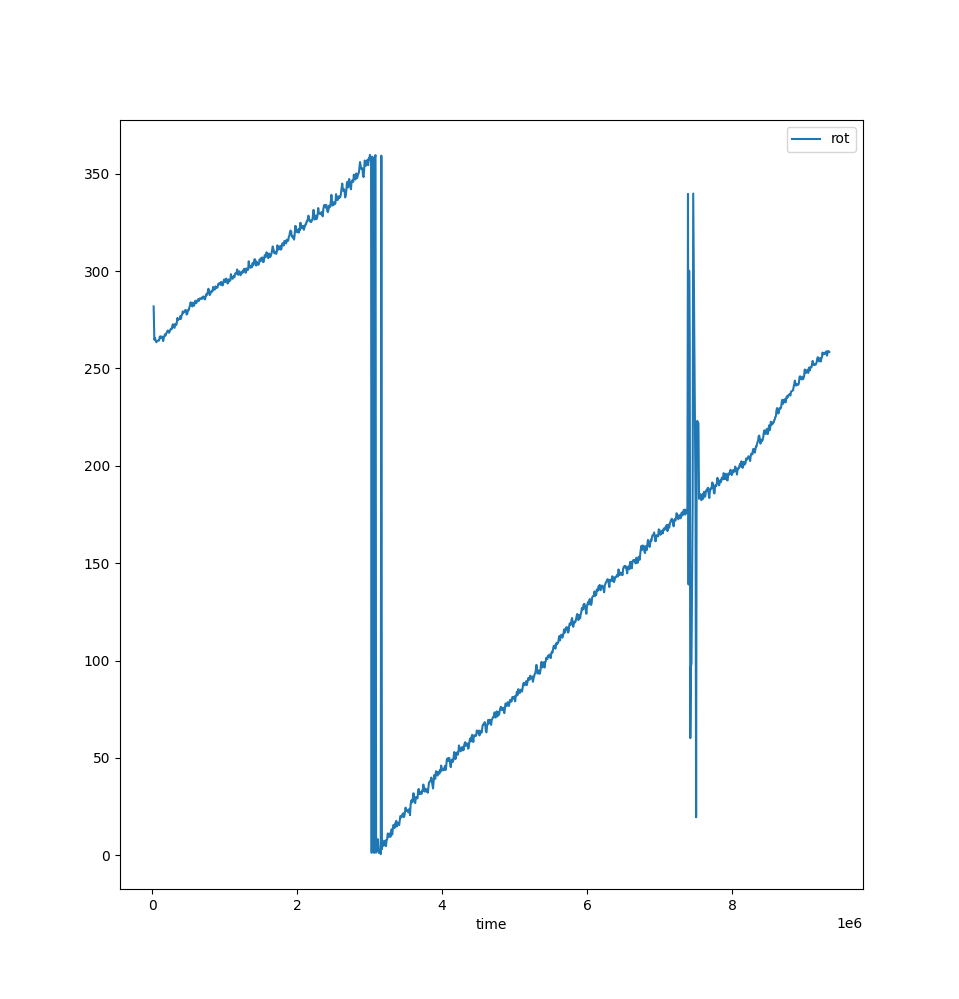
\includegraphics[width=\linewidth]{lernportfolio_assets/CompassRotation360.png}
      \caption{Y-Achse: Rotation in Grad\newline}
    \end{subfigure}
    \begin{subfigure}{0.45\linewidth}
      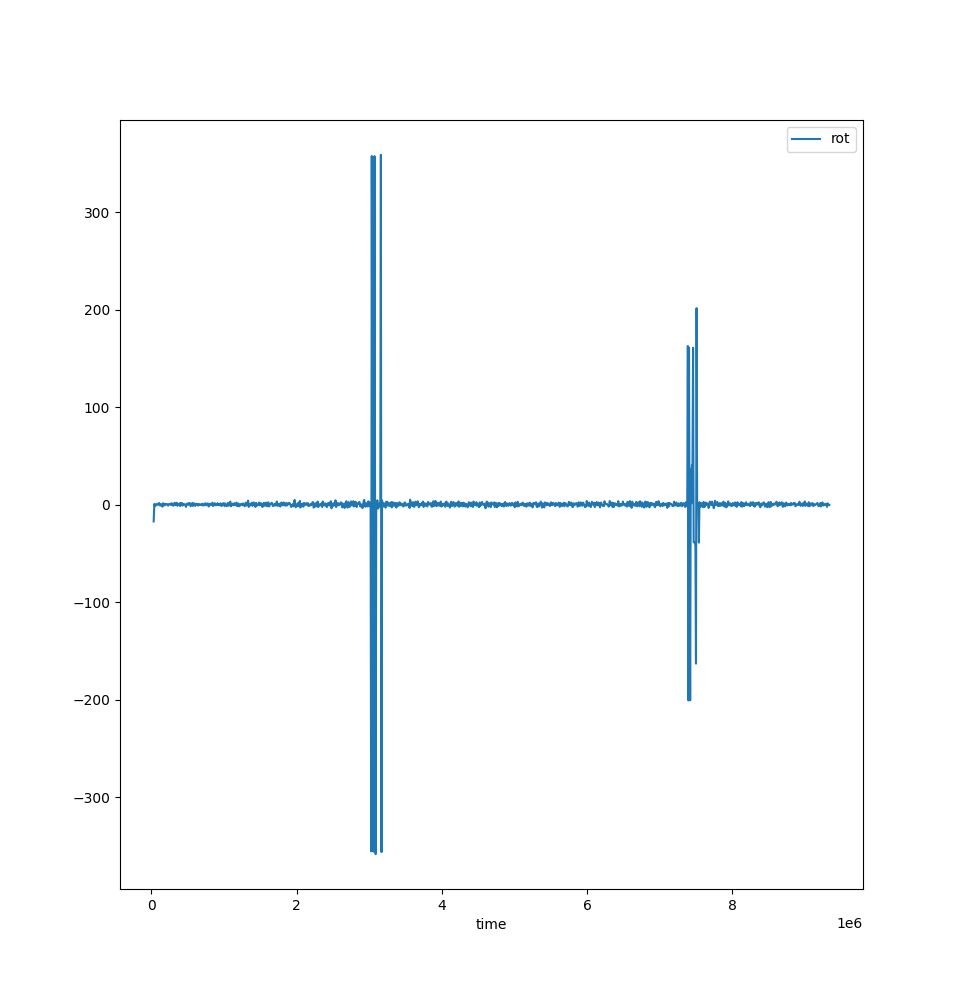
\includegraphics[width=\linewidth]{lernportfolio_assets/CompassRotation360Diff.png}
      \caption{Y-Achse: Differenz von Messpunkt n+1 zu Messpunkt n in Grad}
    \end{subfigure}
    \caption{X-Achse: Zeitverlauf ohne Einheiten aber mit konstanter Änderungsrate}
  \end{figure}

  Nach berechnen des Mittelwertes sieht man, dass Ausreißer eliminiert werden
  konnten. In dem Abschnitt im Intervall von 7365036 bis 7557114 kam es zu
  einer Fehlfunktion des Sensors. Dieses kann man in den Rohdaten sehr klar
  erkennen:\\
  \\
  \begin{tabular}{lr|lr}
    \centering
    Zeit    &  Rotation & Zeit    &  Rotation \\
    7373037 &  175.8100 & 7461065 &  339.8530 \\
    7381039 &  176.9410 & 7469066 &  301.4020 \\
    7389039 &  339.6910 & 7477074 &  262.9910 \\
    7397040 &  139.0360 & 7485076 &  224.1490 \\
    7405049 &  300.2140 & 7493077 &  182.4500 \\
    7413051 &  260.7380 & 7501077 &   19.5078 \\
    7421052 &   60.1572 & 7509085 &  221.1170 \\
    7429053 &   96.8943 & 7517087 &  223.1090 \\
    7437062 &   98.4091 & 7525089 &  222.1960 \\
    7445063 &  138.8670 & 7533090 &  221.9140 \\
    7453064 &  178.8960 & 7541103 &  183.0830 \\
  \end{tabular}
  \\

  Das starke Schwanken der Linie im ersten Teil entsteht durch den Sprung
  von 0 auf 360 Grad. Die Rohdaten enthalten hier keine größeren Störungen. Es
  ist daher ein rein visueller Effekt.

  %TODO Grad zu Zeichen
  Eine Zeitdifferenz von 176.075 Einheiten ist 0,14 Sekunden.
  Mit einer Standardabweichung von 83.22\si{\degree}, einem Minimum von 19.5\si{\degree} und
  einem Maximum von 339.85\si{\degree} ist dieser Abschnitt sehr inhomogen.

  Bei Betrachtung der Differenz eines Messwertes zu dem nächsten innerhalb eines
  vermutlich homogenen Abschnittes mit zeitlicher Kohärenz - hier der
  Abschnitt von 4002107 bis einschließlich 4119625, was 0,095 Sekunden sind -
  gibt es eine Standardabweichung von 1,58\si{\degree}. Der Bereich zwischen Minimum
  und Maximum umfasst 6,25\si{\degree}. Damit ist dieser exemplarische Bereich relativ
  homogen. Jedoch kann es durch die Abweichung vom Mittelwert von bis zu $\pm
  3$\si{\degree} auch in diesen Bereichen zu zu frühem bzw. spätem Stoppen kommen.
  \\
  \begin{tabular}{lr}
    {} &        rot \\
    mean  &   0.066956 \\
    std   &   1.585327 \\
    min   &  -2.960200 \\
    25\%   &  -0.919675 \\
    50\%   &   0.193750 \\
    75\%   &   0.954975 \\
    max   &   3.298600 \\
  \end{tabular}
  \\

  Die Wahl des gleitenden Mittelwertes ist, aus der Retroperspektive heraus
  betrachtet, die falsche Wahl. Hierdurch konnten Fehler des Sensors nicht abgefangen
  werden. Unter der realitätsnahen Annahme, dass die Geschwindigkeit und damit
  die Drehung sich für den Buggy durch eine lineare Funktion annähern lassen
  kann, ist die Beschreibung der Rotation durch ein lineares Regressionsmodell möglich.
  Durch dieses könnte man die aktuellen Richtung mit der Vorhersage des
  Regressionsmodelles vergleichen und bei zu großer Inkongruenz den Messwert als
  Fehler verwerfen und anschließend die Richtung aus dem Regressionsmodell und der
  Veränderung in der Motorsteuerung berechnen.
  Zudem hat sich in den Tests gezeigt, dass der Buggy unterstützt durch den
  Sensor lediglich inkonsistent bei der Drehung um einen vorgegebenem Winkel ist.
  Insgesamt ist die Genauigkeit des Sensors mäßig. Fehlmessungen kommen vor.

  \end{subsection}
  \begin{subsection}{Integration in das Programm}
    Der Sensor wird vorallem bei dem automatischem Fahren - implementiert in der
    Klasse "`automatic\_movement"' - genutzt. Durch die
    Richtungsdaten können Drehungen um einen Winkel vollzogen werden. Diese
    Fähigkeit des Buggys wird in den Videos "`RechteckWinkel.mp4"' zur Schau
    gestellt. Der Buggy soll 4 mal 20 cm forwärts fahren und sich dann um 90
    Grad drehen. Die Drehung um 90 Grad funktioniert mäßig.

    Eine Interpretation des Winkels als Richtungsvektor ermöglicht die
    Fortbewegung im Raum auf Grundlage von Vektorarithmetik.
    Ein Beispiel ist hierfür das Video "`AutomatischesUmfahrenGegenstand.mp4"'.
    Die Startrichtung des Vektors wird als (0,1) und die Startposition des
    Buggys als (0,0) vorgegeben. Ziel des Buggys ist es zu dem Punkt (0, 120) zu fahren.
    Stößt der Buggy auf ein Hindernis untersucht er die linke Umgebung, bis das
    Objekt nicht mehr im Weg steht und fährt 30 cm an dem Hindernis vorbei.
    Danach richtet der Buggy sich erneut zum Ziel aus und bewegt sich weiter.
    Könnte der Buggy das Hindernis auf der linken Seite nicht ausweichen, würde
    er auf der rechten Seite gleiches probieren.
    Bei erfolgreicher Ankunft am Ziel stoppt der Buggy.

    Das Abfahren eines Rechteckes basierend auf einer Abfolge des Abfahrens von
    Punkten ist in den Videos "`RechteckPunkte.mp4"' zu sehen.

    Der Buggy kann zudem beim geradeaus fahren die Startrichtung halten. Dieses
    ist im Video "`RichtungHalten.mp4"' zu sehen.

    Desweiteren kann der Buggy, wie im Video "`Kurve180.mp4"' demonstriert,
    Kurven abfahren.
  \end{subsection}
\end{section}

\begin{section}{Zusammenfassung}
  \begin{subsection}{Zusammenfassung Leonhard Kipp}
    In der Projektphase ist mir bewusst geworden, dass Sensoren nicht nur
    fehleranfällig sind, sondern dass die Analyse und Aufbereitung der Inputs
    von Sensoren sowie das Abfangen falscher Messdaten sehr viel mehr Zeit in Anspruch nimmt und weitaus komplexer
    ist als die Implementation der Abfragen der Sensoren in Software. Die
    hierfür benötigte Zeit habe ich unterschätzt.
    
    Bei der Aufbereitung der Messdaten ist die Bildung eines Durchschnittes nicht
    immer das beste Mittel. Das arithmetische Mittel sowie die
    Standardabweichung ist anfällig gegenüber Ausreißern
    in den Daten. Eine bessere Messmethode für die Betrachtung von wenigen Daten
    kann die Verwendung des Medians und der Mittleren absoluten Abweichung vom
    Median sein.

    Zudem hat die Projektphase das Verständnis von Datenblättern gefördert. Ich
    fühle mich mittlerweile sehr viel schneller und sicherer im Umgang mit diesen.

    Eine Auffrischung bzgl. der Mathematik war das Anwenden von Vektorarithmetik. Das Vorstellen,
    welche Bewegungen der Buggy durch die implementierten Funktionen vollziehen
    wird, hat gleichzeitig das räumliche Vorstellungsvermögen trainiert.

    Was ich nicht vergessen werde ist, dass
    \begin{lstlisting}
      std::cout << calculated_float_value << std::endl
      ...Later on taking, acos returning NaN
      std::cout << std::acos(calculated_float_value) << std::endl
    \end{lstlisting}
    1 ausgeben mag, aber der arcus cosinus dennoch NaN zurück gibt.
    Die Rechnung war korrekt, jedoch hat der Computer aufgrund der geringen
    Präzision einen Wert minimalst größer als eins produziert. Das Terminal hat
    diesen Wert aufgrund seiner geringen Differenz zu eins als eine eins interpretiert.
    Diesen Fehler zu finden, war Nerven zerreibend.

    Beim nächsten Mal würde ich die Klassen "`vertex2D"' und "`degree "' nicht
    selber implementieren. Auch wenn die Implementation vermeintlich "`trivial"'
    erscheint, schafft man es dennoch zu übersehen, dass man an einer Stelle die
    Wurzel nicht hätten ziehen dürfen. Die Implementations- und Fehlersuchzeit
    wiegt das Installieren und die Einarbeitung in eine Mathebibliothek nicht
    auf. Des Weiteren kann man die Bibliothek in anderen Projekten
    wiederverwenden.
    Durch die eigen Implementation war man gezwungen nochmals
    intensiver über die Mathematik hinter den Funktionen nachzudenken. Man kann
    dieses als Lernanreiz oder als kognitive Last auffassen.

    Darüber hinaus würde ich beim nächsten Mal versuchen, die \wiringPi{}
    Bibliothek auf meinem Rechner statisch zu linken, damit ich eine
    erfolgreiche Kompilierung vor dem Hochladen des Codes auf den RaspberryPi
    sicherstellen kann. Das Ausbessern von Fehlern über SSH in einem ungewohntem
    Texteditor ist unkomfortabel.

    Die Verwendung von WhatsApp als Kommunikationsplattform war die falsche
    Wahl. Gibt es mehrere Aufgaben gleichzeitig zu koordinieren, verliere ich in
    einem linearen Nachrichtenstrom schneller die Übersicht über den Stand jeder
    einzelnen Aufgabe als in Foren bzw. Themen basierten Kommunikationsplattformen.

    Beibehalten würde ich die Verwendung eines RaspberryPi's und das Schreiben
    des Lernportfolios mit \LaTeX. Das Verbinden
    können über SSH, die Rechenleistung und in einer gewohnten Umgebung
    (Bash-Shell) zu sein, hat seine Vorteile gegenüber einfacheren Microcontrollern.
    Der Vorteil von \LaTeX\ besteht vor allem darin, dass es aus \gquotes{plain text}
    besteht und daher sich sehr einfach mit Git verwalten lässt.

    Das meiste habe ich in dem Umgang mit den Sensoren gelernt. Das Lesen der
    Datenblätter und die Implementation von Sensorabfragen waren für mich Neuland.

    Spaß hat mir die Datenanalyse und Datenaufbereitung gemacht. Die Erstellung
    eines kleinen ncurses basierten Benutzerinterfaces hat mir aufgezeigt, wie
    graphische Terminalprogramme implementiert sein mögen und hat so seinen
    eigenen Reiz gehabt. Zu sehen, wie die implementierten Funktionen
    aufgrund von Ausreißern in den Messwerten zu falschem Verhalten neigen,
    waren Tiefpunkte in der Arbeit. Zugleich war es das am meisten
    Motivierenste, wenn man durch Transformationen, wie die Bildung des
    Mittelwertes oder eines gleitenden Mittels, das Verhalten der Funktionen
    verbessern konnte.
       
  \end{subsection}
  \begin{subsection}{Zusammenfassung Jens Dennigmann}
  Durch die Projektphase ist mir wieder bewusst geworden, dass Kommunikation durch 
  Messenger besonders am Anfang der Phase relativ schwerfällig ist. Dazu kommt noch der 
  mangelnde persönliche Kontakt, der besonders am Anfang einer Projektphase zur Organisation 
  wichtig ist, aber durch die Umstände dieses Semesters wegfiehl. Eine bewusstere 
  Entscheidung für eine Kommunikationsplattform hätte hier wahrscheinlich bei einigen 
  Startschwierigkeiten geholfen.
  
  Weitere Punkte bei denen ich viel gelernt habe, waren vorallem der Umgang mit Datenblättern 
  und das Testen von Sensoren. Durch das selbständige Arbeiten mit z.B. dem Datenblatt zum 
  Magnetsensor habe ich gelernt zu unterscheiden zwischen Abschnitte, auf die
  man achten muss und Abschnitte, die eher unrelevant für einen sind. Mir zeigt
  sich, dass man nicht direkt zu den gewünschten Registern springen sollte, sondern auch 
  allgemeinere Erklärungen zuvor für einen relevant und wichtig sind.
  
  Beim Testen von dem Magnetsensor fiel mir schnell auf, wie wichtig Funktionen sind mit denen 
  man schnell viele Testdaten bekommt. Die Daten von dem Sensor sahen anfangs recht willkürlich 
  aus und erst nach dem Auswerten von einigen Testdaten konnte man sehen, dass sich eine 
  Ellipse formt. Die Anfälligkeit für Störungen konnte man sehen. Selbst bei
  relativ störungsfreiem Testen sind die Werte nicht immer präzise.
  
  Es gab auch ein paar Sachen die leichter fielen als erwartet. So z.B. das
      Anschließen von dem Magnetsensor oder das Verbinden zum Raspberry Pi, das mit dem Programm Putty relativ simpel 
      und angenehm gemacht ist. 

      Anschließend lässt sich noch sagen, dass besonders das Arbeiten, mit dem Buggy direkt bei 
      einem selber vor Ort, Spaß gemacht hat. Das schnelle Erkennen von Resultaten hat sehr dazu 
      motiviert weiter zu arbeiten und Ziele zu erreichen. Auch das arbeiten mit Github, was 
      %Unser Projekt war ein mini Projekt
      mittlerweile recht selbstverständlich ist, besonders bei größeren Projekten wie diesem, hat 
      sehr geholfen. Man konnte den Code der Gruppenmitglieder schnell selber einsehen und sich 
      auch so gegenseitig helfen und austauschen.
  \end{subsection}
        \begin{subsection}{Zusammenfassung Pierre Dahmani}
            % Start task 5.1 of Arbeitsauftrag Projektphase_EES.pdf
            % Beschreiben Sie kurz, was Sie in der Projektphase bei der Arbeit mit
            % dem Buggy gelernt haben.
            \begin{paragraphwithnewline}{Gelerntes durch Arbeit mit dem Buggy}
            Beim wiederholten Messen von Signalen innerhalb kürzester Zeit muss
            man die Slew-Rate in betracht ziehen um falsche Werte zu verhindern.
            Sensoren sind zwar ziemlich genau, jedoch weit davon entfernt, perfekt
            zu sein. Bei einzelnen Messungen kenn eine hohe Varianz entstehen, welche
            durch das Bilden eines Mittelwerts niedrig gehalten werden kann. Man muss
            beachten, dass einzelne Messungen durch Störfaktoren komplett falsche Werte
            liefern können, die man aussortieren muss um das Ergebnis nicht zu 
            verfälschen. Wenn man Probleme mit dem Code hat kann es sehr hilfreich
            sein die Teammitglieder zu befragen. Damit die Teammitglieder den eigenen
            Code verstehen ist es sehr wichtig diesen gut zu Dokumentieren und
            beschreibende Funktionen und Variablennamen zu wählen. Gemeinsam an
            einem Projekt zu arbeiten ist schwieriger als zu Beginn erwartet. Die in
            der Vorlesung gelernte Methodik des Code Reviews hat sich als sehr hilfreich
            bewiesen. Dies haben wir konsequent über GitHub anhand von Pull-Requests
            durchgeführt.
            % End task 5.1
            \end{paragraphwithnewline}

            % Start task 5.2 of Arbeitsauftrag Projektphase_EES.pdf
            % Was würden Sie beim nächsten Mal anders machen? Was würden Sie
            % beibehalten?
            \begin{paragraphwithnewline}{Konsequenzen für zukünftige Projekte}
            Beim nächsten Mal sollten wir mehr Zeit in die Aufgabenplanung stecken
            und rechtzeitig Feedback geben und um Hilfe bitten, wenn etwas nicht
            funktioniert wie geplant und man dadruch nicht voran kommt. Wir müssen
            darauf achten dass einzelne Gruppenmitglieder den Buggy nur haben, wenn
            sie auch Zeit haben sich um die Aufgabe zu kümmern. Was wir beibehalten
            würden ist die Aufgabenverteilung. Wir sind zu dritt und konnten dadurch
            für jeden Aufgabenbereich einen spezialisten wählen, der dafür verantwortlich
            war, dass die Funktionalitäten ausgebessert und gefundene Fehler behoben wurden.
            Das Verwenden von GitHub als VCS war eine gute Wahl weil jeder der
            Teammitglieder bereits vertraut damit war. Das wählen von \LaTeX\xspace
            für die Erstellung des Lernportfolios hat zu Beginn viel Zeit in Anspruch
            genommen. Durch die Steile Lernkurve und gegenseitige Unterstützung war
            es im Nachhinein jedoch seine sehr gut Entscheidung, die wir für kommende
            Portfolios beibehalten werden. Die Kommunikation über WhatsApp hat uns
            einen leichten Einstieg in die Zusammenarbeit gegeben. Jedoch wäre eine
            andere Wahl der Kommunikation besser gewesen. Beim nächsten Projekt würden
            wir das anders angehen. Wir haben uns überlegt die GitHub spezifischen
            Features zur Projektplanung zu nutzen. Dadurch bekommt man einen Problem
            spezifischen Einblick zu den Fragen und kann direkt den jeweiligen Issue
            oder Codeabschnitt einsehen. Es werden ebenfalls nicht alle beteiligten
            Benachrichtigt, wenn die Frage nur an eine Person gehen soll. Dadurch wird
            der leicht enstehende Spamm bei WhatsApp verhindert.
            \end{paragraphwithnewline}
            % End task 5.2

            % Start task 5.3 of Arbeitsauftrag Projektphase_EES.pdf
            % Bewerten Sie, in welchen Teilen der Aufgabenstellung Sie viel gelernt
            % und welche Ihnen Spaß gemacht haben.
            \begin{paragraphwithnewline}{Das hat uns Spaß bereitet}
            Am meisten Spaß hat es gemacht den implementierten Code dann am Buggy zu
            testen. Auch wenn die Messungen einen stellenweise zur Weißglut gebracht
            haben hat man dadurch gelernt auf wie viele Faktoren man bei Sensoren
            achten muss und was alles schief gehen kann. Durch die Projektphase
            haben wir ein besseres Verständnis dafür bekommen, wie man Treiber
            programmiert und diese schließlich verwendet. Wir haben erstaunlich
            viel Spaß daran gehabt und wollen uns in unserer Freizeit nun vermehrt
            mit dem Thema embedded Pi auseinandersetzen.
            \end{paragraphwithnewline}
            % End task 5.3
        \end{subsection}
\end{section}

\begin{thebibliography}{9}

    \bibitem{motorhatDownloads}
        Schematas des Motorhats
        \url{https://learn.adafruit.com/adafruit-dc-and-stepper-motor-hat-for-raspberry-pi/downloads}
        Zuletzt abgerufen am: 25.05.2020

    \bibitem{datasheetPCA9685}
        Datasheet PCA9685 PWM driver,
        \url{http://www.adafruit.com/datasheets/PCA9685.pdf},
        Zuletzt abgerufen am: 25.05.2020

    \bibitem{datasheetTB6612}
        Datasheet TB6612 Motor driver,
        \url{http://www.adafruit.com/datasheets/TB6612FNG_datasheet_en_20121101.pdf},
        Zuletzt abgerufen am: 25.05.2020

    \bibitem{referenzcode}
        adafruit-motor-hat-cpp-library,
        Autor tomfclarke,
        \url{https://github.com/tomfclarke/adafruit-motor-hat-cpp-library},
        Zuletzt abgerufen am: 25.05.2020


    \bibitem{datasheetUltrasonic1}
        Datasheet HC-SR04,
        \url{https://www.electroschematics.com/wp-content/uploads/2013/07/HCSR04-datasheet-version-1.pdf},
        Zuletzt abgerufen am: 25.05.2020
    \bibitem{datasheetUltrasonic2}
        Datasheet HC-SR04,
        \url{https://components101.com/ultrasonic-sensor-working-pinout-datasheet},
        Zuletzt abgerufen am: 25.05.2020
    \bibitem{datasheetUltrasonic3}
        Datasheet HC-SR04,
        \url{https://cdn.sparkfun.com/datasheets/Sensors/Proximity/HCSR04.pdf},
        Zuletzt abgerufen am: 25.05.2020

    \bibitem{datasheetMagnet}
        3-Axis Magnetic Sensor QMC5883L,
        \url{https://www.ili.fh-aachen.de/goto_elearning_file_554919_download.html},
        Zuletzt abgerufen am: 25.05.2020

    \bibitem{forumMagnet}
        3-Axis Magnetic Sensor QMC5883L,
        \url{https://forum-raspberrypi.de/forum/thread/39028-qmc5883l-kompass-daten-konvertieren/},
        Zuletzt abgerufen am: 25.05.2020

    \bibitem{wiringPi}
        wiringPi Bibliothek
        \url{http://wiringpi.com/},
        Zuletzt abgerufen am: 25.05.2020

        % \bibitem{}
        %   Datasheet HC-SR04,
        %   \url{https://en.wikipedia.org/wiki/Speed\_of\_sound},
        %   Zuletzt abgerufen am: 25.05.2020
        % \bibitem{datasheetUltrasonic1}
        %   Datasheet HC-SR04,
        %   \url{http://www.sengpielaudio.com/calculator-speedsound.htm},
        %   Zuletzt abgerufen am: 25.05.2020

\end{thebibliography}

\pagebreak
\begin{section}{Selbstständigkeitserklärung}
    Hiermit erklären wir, dass wir die Projektarbeit selbstständig und ohne
    unerlaubte fremde Hilfe angefertigt, keine anderen als die
    angegebenen Quellen und Hilfsmittel verwendet und die den verwendeten Quellen
    und Hilfsmitteln wörtlich oder inhaltlich entnommenen Stellen als solche kenntlich
    gemacht haben.
\end{section}

\end{document}
